\chapter{Evaluation Experiments and Results}
\label{sec:results}
\thispagestyle{fancy}
The system has been evaluated on the TIME collection (\cite{TIME}) provided by the course staff. The collection consist of 423 documents and 10 queries with specified relevant documents.

\section{Basic System}
The basic system has been evaluated using only precision and recall, no performance considerations has been made. The results from a default implementation using cosine scoring mode are demonstrated by Figure \ref{fig:cosine}. The figure plots a line for each of the queries, $x$ and $y$ axis correspond to recall and precision, and point $i$ on each line correspond to a (precision,recall) value after inspecting top $i$ results. The diagram plots up-to 50 top results for each query.

The diagram is quite easy to understand by keeping in mind that a correct result will either increase both the precision and recall or keep them at 1.0. After the maximum number of correct results is achieved, the recall will stay at 1.0, while precision will drop. Wrong results always result in a drop in precision, while the recall value is kept at the same level.

As Figure \ref{fig:cosine} shows, the total search quality is somewhat poor - for two out of ten queries the first result is already irrelevant, and the highest possible recall value at precision level 1.0 is 0.6, while it is impossible to achieve a precision higher than 0.6 for a recall level at 1.0. The best combination of precision and recall altogether is slightly off (0.8, 0.8)

\begin{sidewaysfigure}[h]
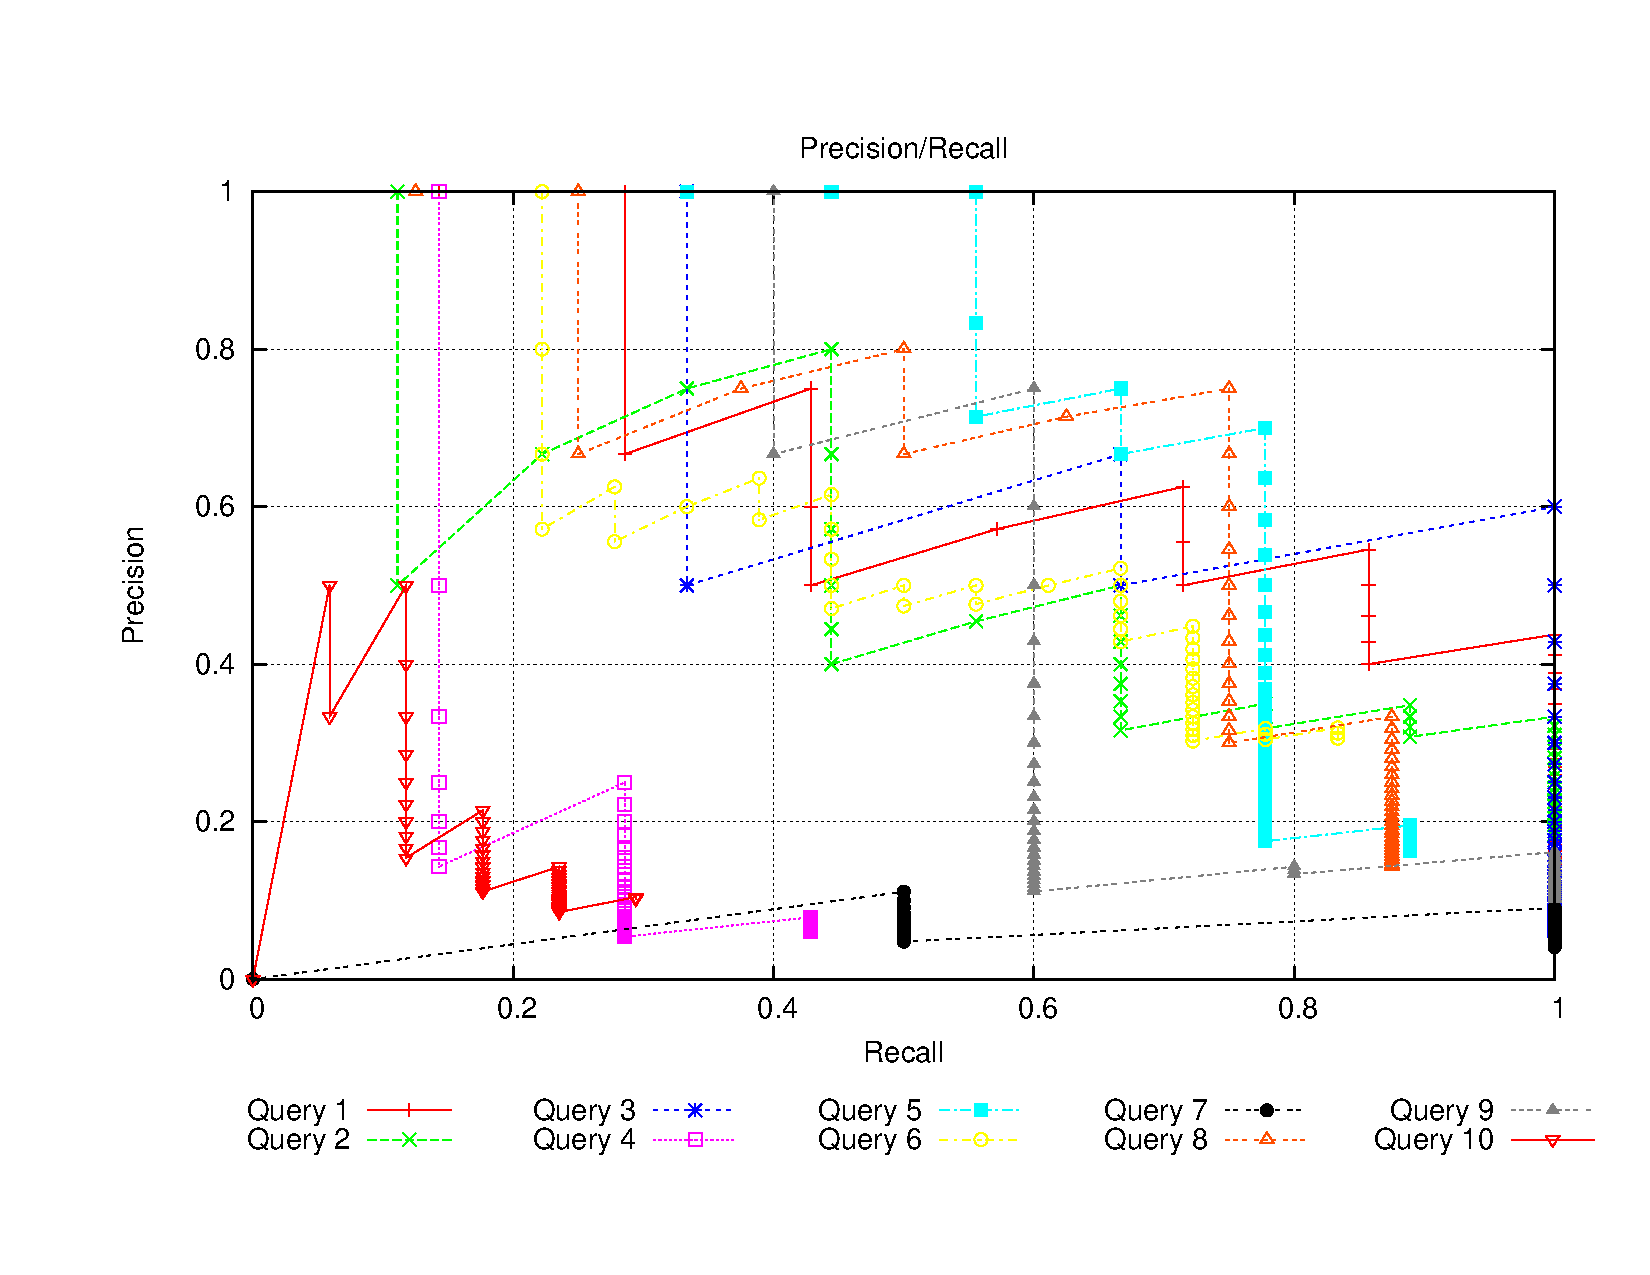
\includegraphics[width=1.0\textwidth]{include/bench_cosine}
\caption{Evaluation Results with Cosine Scoring Model}
\label{fig:cosine}
\end{sidewaysfigure}

As the Okapi BM-25 has also been implemented, it was quite interesting to evaluate its performance against the cosine model. As Figure \ref{fig:okapi} shows, Okapi results in a great quality improvement. Only one query fails to on the correct top results, but it contains both correct results within top five results. Most of the queries success to achieve a combine recall-precision value greater than (0.7, 0.7), and most important one of the queries success also to achieve a value at (1.0, 1.0), while the worst performance (observed for query number four) is just the same as for the cosine model.

\begin{sidewaysfigure}[h]
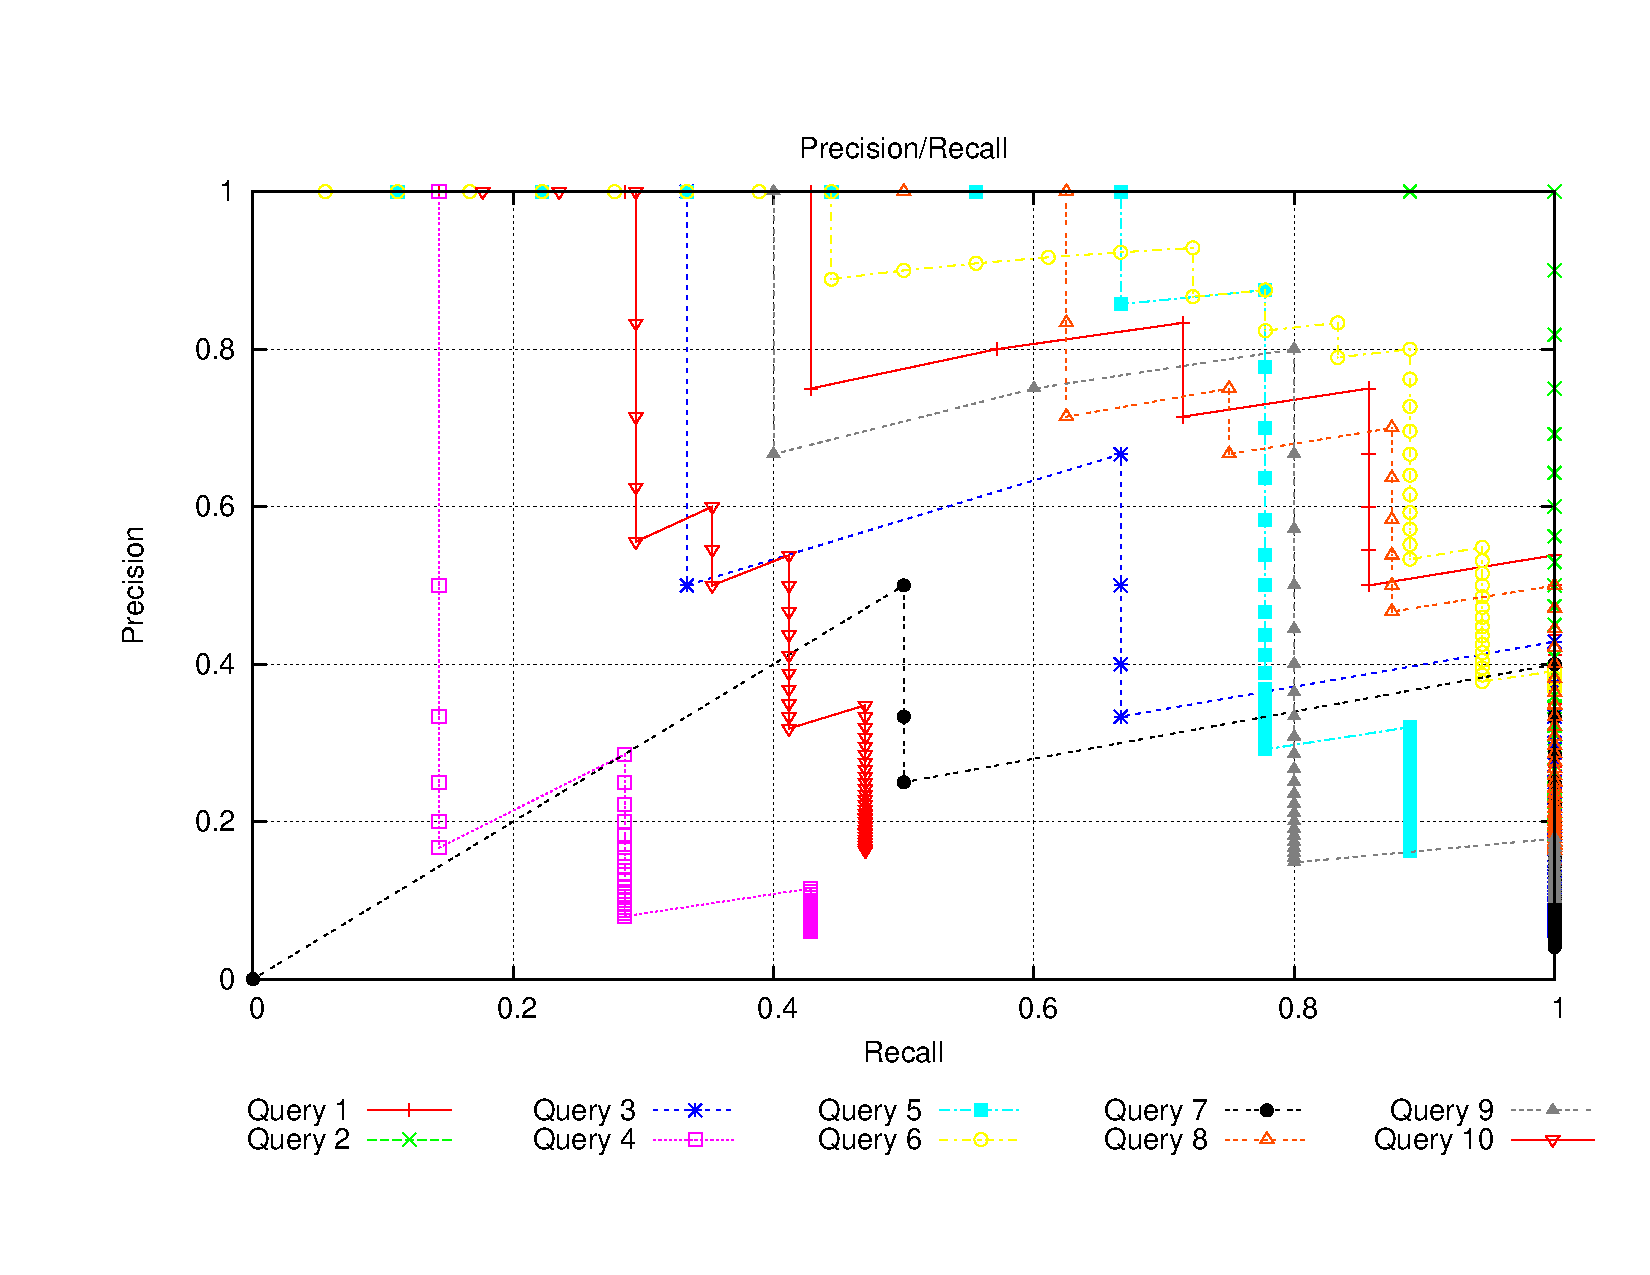
\includegraphics[width=1.0\textwidth]{include/bench_okapi}
\caption{Evaluation Results with Okapi BM-25 Model}
\label{fig:okapi}
\end{sidewaysfigure}

\section{Extended System}

It is hard to fairly evaluate the success of a clustered results versus a non-clustered result, papers like \cite{zamir} usually compare the results to other clustering algorithms. There are several reasons for this. First, the clustered result contains information that the non-clustered result does not contain (the name of the cluster, the knowledge that the results are clustered together). Secondly, if standard precision/recall evaluation is used, several problems arise. The most important is in which order the results should be tried. Since the course of action for a human user using a clustered result would be to first check the label of the cluster, and then check the results, evaluation of the results only would not make sense. Whatever is done to evaluate the results will need human interaction. 

Evaluating simple queries with suffix tree clustering shows that short queries are usually the best when trying to find good clusters. With longer queries, there are more "garbage" nodes, which not necessarily contains documents which should be clustered together.

Because of the problems with using standard precision/recall to score clustered queries, as well as suffix tree clustering not being good on long queries (and the queries in the test set was quite long), it was chosen not to do a quantitative test with the suffix tree clustering method. 

If a simple qualitative test is done, by doing random queries like "buddhist", "war" or "britain", many (but not all) of the clusters that are returned have articles that are grouped together. The examples can be seen in \ref{fig:clusterresults}.

\begin{table}
\begin{tabular}{|l|p{0.8\textwidth}|}
\hline
Query & Clusters \\
\hline
buddhist & \{"south viet nam roman catholic president ngo dinh diem" "quang duc" "buddhist monk" "virtual martial law" "flag" "religious freedom"\}, \{"diem government" "buddhist leaders"\}, \{"sister law mme ngo dinh nhu" "ngo dinh nhu has" "mme nhu has banned" "diem brother" "nine" "church" "buddhist schools"\}\\ \hline
war & \{"war south viet nam" "viet cong"\}, \{"international red cross"\}, \{"government"\}, \{"mekong delta" "diem"\}, \{"various" "sino soviet split" "maneuver" "lenin"\}, \{"mao tse tung"\}, \{saudi arabia jordan" "egypt saudi arabia" "imam" "yemeni" "war yemen" "saudi arabia has" "sallal" "tribesmen" "veteran" "badr" "egyptian" "san" "team" "limit" "wide" "little war"\}\\ \hline
britain & \{"osteopath stephen ward" "profumo case" "john profumo was" "mentor" "christine keeler" "trial charges"\}, \{"government"\}, \{"harold macmillan"\}, \{"national"\}, \{"intention" "common market britain" "efta" "tariff" "outer" "regard" "join"\},\{"sir alec douglas home" "luton" "plain" "proof" "campaign" "seat" "labor years" "next day"\} \\ \hline

\end{tabular}
\caption{Cluster tags for clusters returned in the TIME document set}\label{fig:clusterresults}
\end{table}


The suffix tree implementation still needs a bit of tweaking when it comes to the scoring function that selects the ranking of the clusters, as well as testing with a more diverse data set. However, the clustering method still fulfills its mission, clustering articles with similar subject.